% REV00 Tue 20 Jul 2021 08:12:01 WIB
% START Tue 20 Jul 2021 08:12:01 WIB

\chapter{Kedelapan}

% 11
\begin{figure}[htbp]
% h: here, where the figure appears in the text (use can always just use [h] )
% t: top,  top of the current page.
% b: bottom of the current page.
% p: page, top of the next available float space (sometimes end up being the end of the document).
\centerline{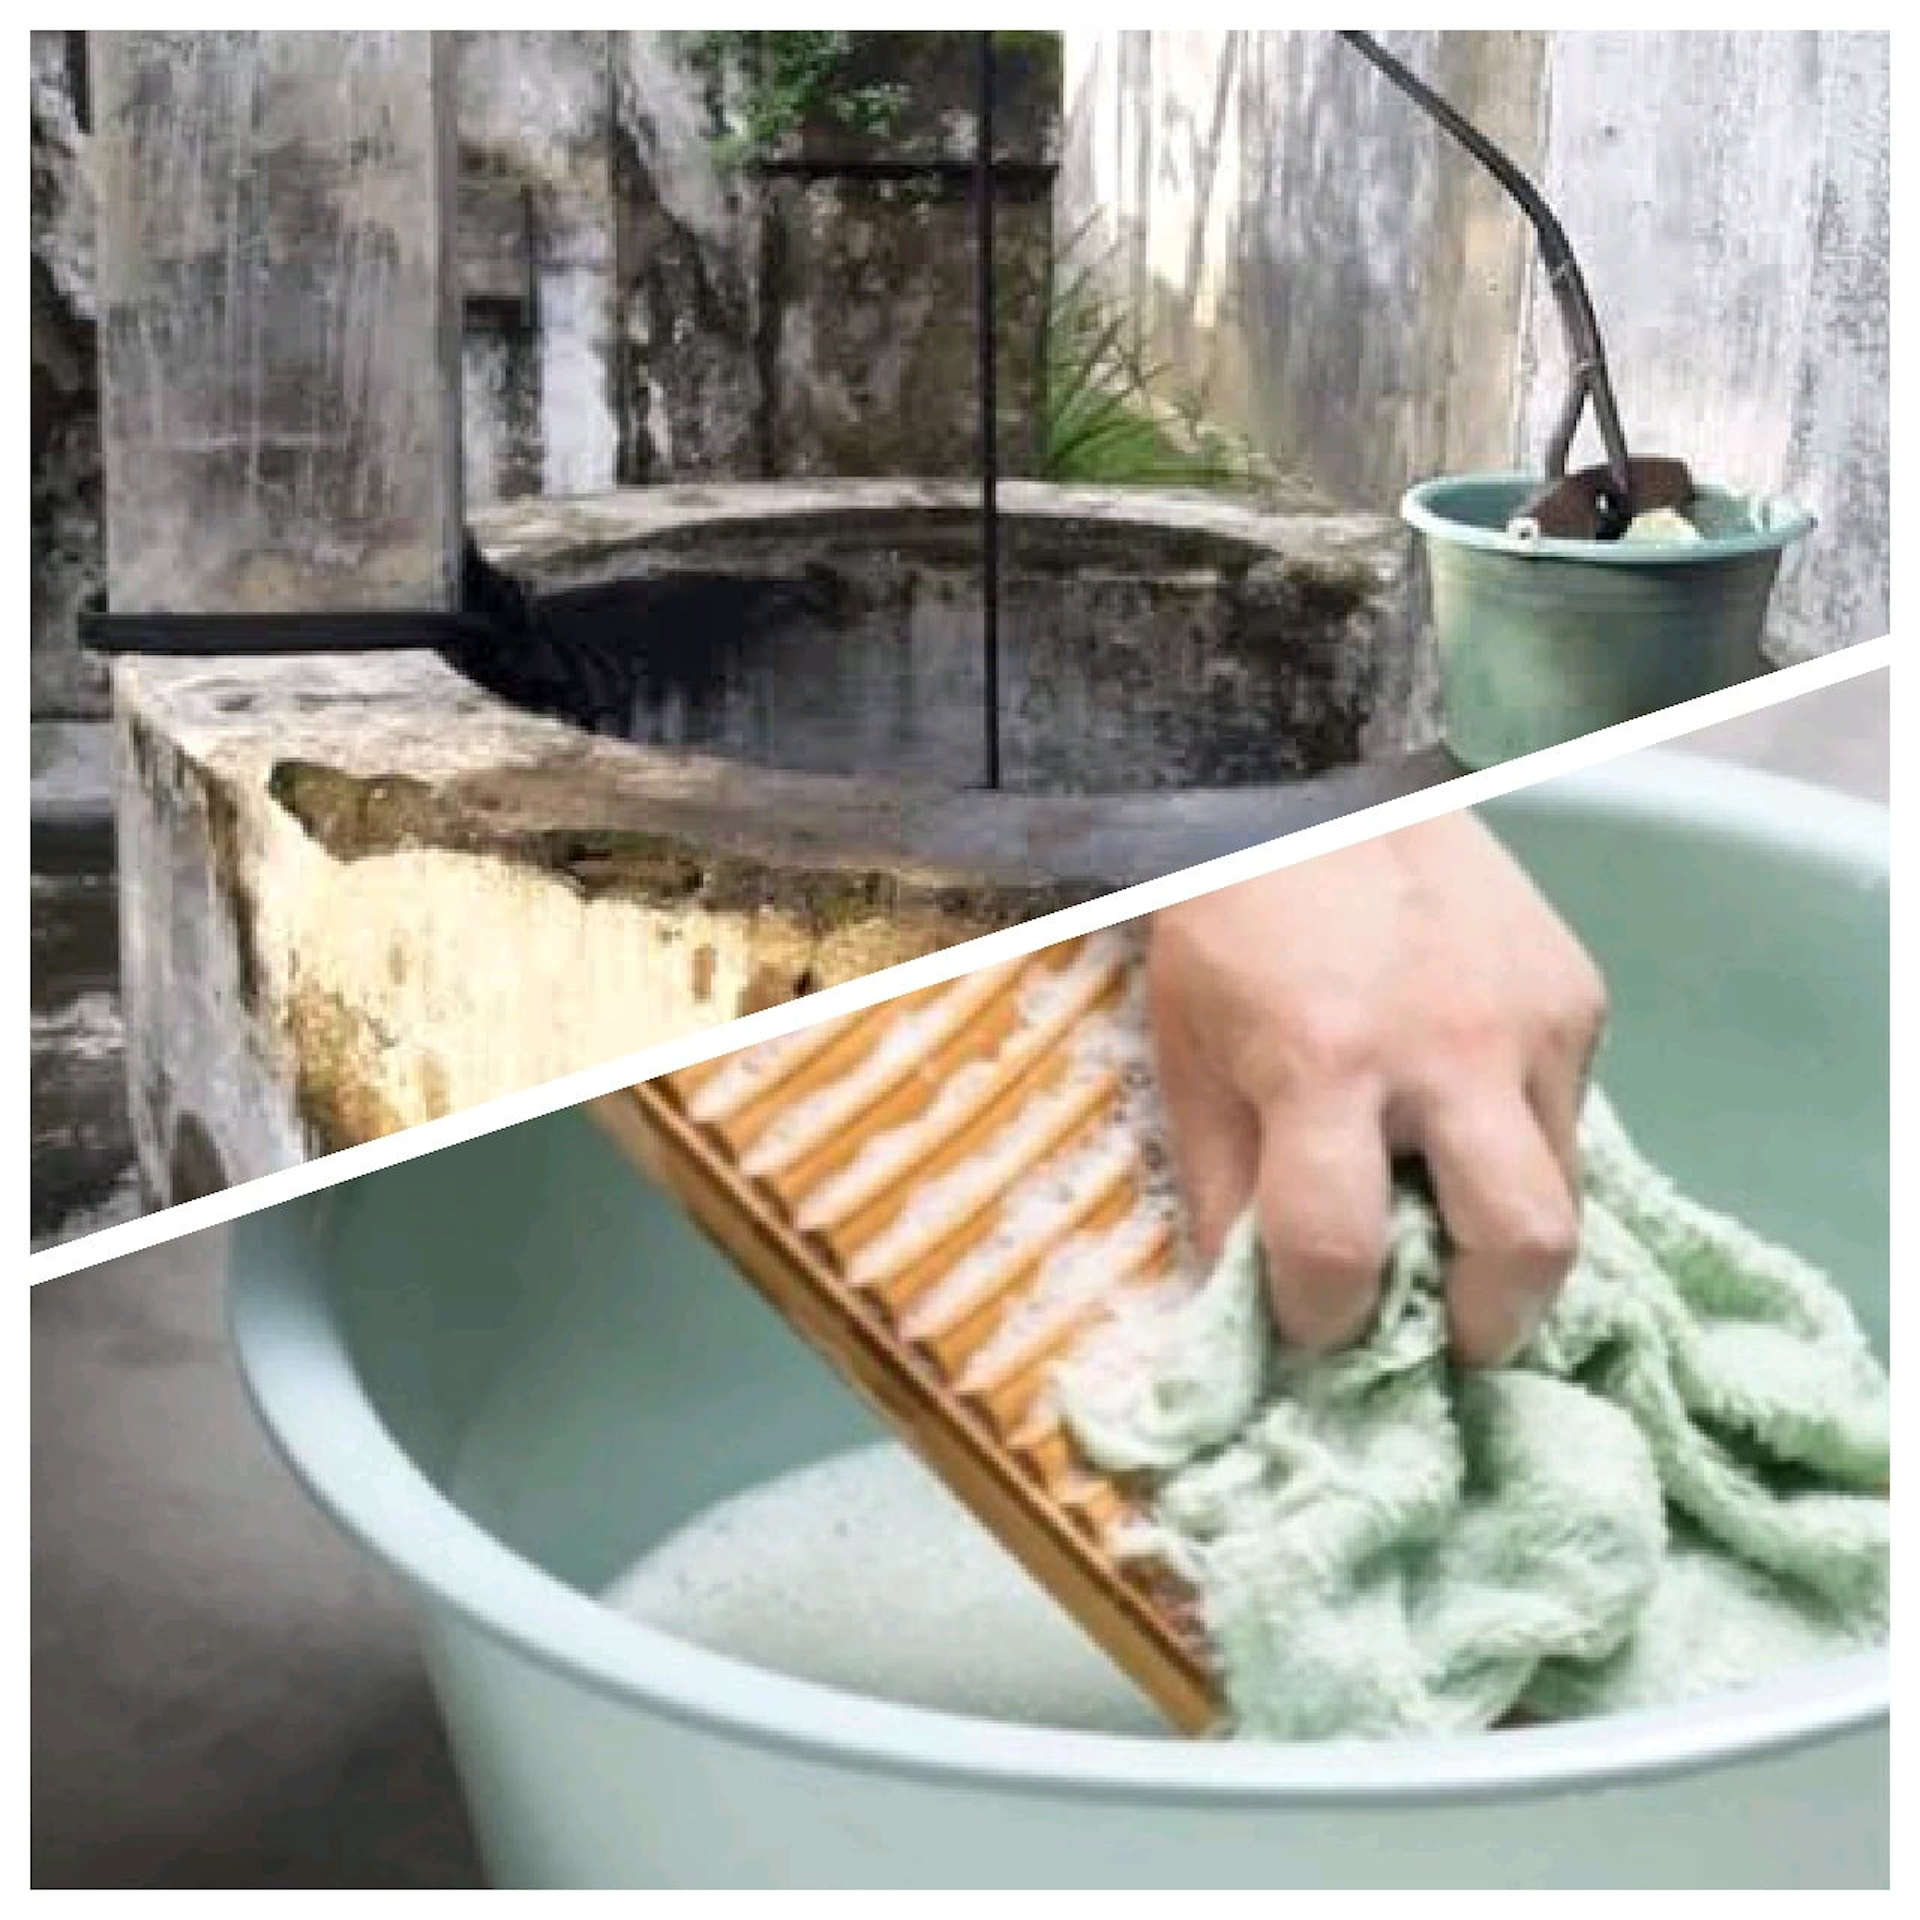
\includegraphics[scale=1.0]{01-08-01}}
\caption{“Ilustrasi sumur timba, dan papan penggilasan”. Sumber: Internet.}
\label{01-08-01}
\end{figure}
%
Jawabannya adalah berdoa kepada Tuhan, banting tulang dan memeras pikiran; ditambah-tambah dengan mencium tangan ibunya setiap pagi dan malam.

Kadang kita terlalu abai untuk dengan mudahnya mengatakan biarlah waktu yang akan meneyelesaikannya. Itu hanya berarti bahwa anda tidak akan pernah siap untuk menerima kekalahan apalagi kemenangan.

Kehadirannya di kampus pada semester-2 menjadi jauh lebih rajin. Tentu perlu sedikit masa untuk sedikit menjauh dari baba maupun mertua. ‘Jauh lebih rajin’ di sini artinya dia ada minggu pertama kuliah, seminggu tiap bulan, dan dua minggu pas ujian akhir. Cukup untuk menunjukkan ke Babanya bahwa dia masih kuliah.

Apa lagi yang harus ditunjukkan? Oke, sukses harus ditunjukkan. Caranya?

Ajukan proposal permintaan dana tambahan untuk biaya praktikum. Beres, uang langsung keluar. Kan ikut anjuran sang Jenderal. Bukti pembayarannya? Gampang. Beli kuitansi tukang sayur, ambil cap-capan himpunan, minta siapa saja tanda tangan (biasanya sobat Bejo selalu mau membantunya!). Tok. Beres. Mana ada staf kantor cabang berani sama ‘anak’ Jenderal?

Langsunglah dia merangsek ke Kings, pertokoan anyar sekitaran alun-alun Bandung untuk membeli sepatu Adidul. Untuk sepatu, seingatku dia hanya mau dua merek saja: Adidas atau Bally. Harus sepatu bagus, katanya, karena perlu banyak jalan kaki. “Bukan cuma buat begaya…”

Dari situ dia bisa berjalan kaki ke simpang jalan ABC-Suniaraja, toko optik dan jam yang legendaris. Dan jam tangan Casio dual-digital pun langsung nempel di tangan kanannya. Seumur hidup, baru pertama kali ada jam tangan di sana. Yang teringat teman-temannya adalah seminggu itu sambil jalan dia selalu memiring-miringkan badannya ke kanan…

“Berat ini jam baru gua…” Huahahahah, teman-temannya ikut bahagia… (Belakangan kenakalan kecil ini harus ia bayar mahal!)

Baba juga melihat Satiri tetap kuliah, dan malah pakai sepatu dan jam anyar warna perak bersinar. Mulailah babanya sedikit cerah, dan menambah-nambah do’a kekuatan buat anaknya. Ibundanya tidak kalah banyak berdo’a untuknya siang-malam. Pada akhir semester-2, nilai-nilai Satiri terbukti lebih tinggi dari nilai-nilainya di semester-1.

What didn’t kill you makes you stronger!

“Baba ini lihat nih, nilai-nilai aye yang sekarang lebih bagus dari sebelon aye kawin…” (Dad, look, my grades this time are a lot better than before I got married…)

Baba semakin tenang. Fitria yang dari rumah gedongan pindah ke rumah Satiri membantu mencairkan suasana. Selepas subuh, ia ‘nimba’ air di sumur dan mencuci pakaian sekeluarga dengan papan ‘penggilasan’ itulah tugas yang ia berikan buat dirinya. Demi suami tersayang.

Pekerjaan seperti itu nyaris tidak pernah ia lakukan sendiri di rumahnya. Berat tetapi menyenangkan. Sementara itu, “ii”, panggilan sayang ibunda Satiri, menyiapkan sarapan pagi ala kadarnya: Singkong atau ubi rebus, atau nasi uduk kalau lagi ada rejeki tambahan.

Hari-hari yang melelahkan namun mebahagiakan itulah yang mebuat dirinya segera hamil. Di usia yang begitu muda. Oia, bahkan ketika menikahpun usianya di KTP harus ditambah angka dua.

Di akhir semester-3, ketika kami ujian Thermodinamika-I, lahirlah putri pertama mereka, dan dengan spontan Bang Tiri kasih nama: Eka Thermikelvi Safira. Anak pertama (eka), lahir waktu ujian Thermodinamika dengan satuan Kelvin, buah cinta Satiri dan Fitria.

What an amazingly beautiful name ya Kelvy Safira

***

Selama kuliah di Bandung, sebetulnya Satiri nyaris tidak punya alamat tetap. Satu-satunya rumah yang pasti baginya adalah di rawa belong, cintanya. Kosan atau kontrakan manapun suka menerimanya. Apalagi rumah di Jl. Gardu Jati 98: Boy, tokoh sakti lainnya dari dunia kangouw Fisika.

Di rumah itu kadang kami mengundang BDU yang hebat itu, atau FPZ yang sekarang profesor fisika, untuk beradu ilmu, eh, minta responsi tambahan.

Sejauh saya mengenalnya, Satiri tidak pernah lebih dari enam hari di Bandung. Pernah memang dia terdesak untuk mengerjakan skripsinya dua minggu di Bandung. Di antara dua minggu musim ujian pun dia memilih ‘terdesak’ pulang ke Rawa Belong, kepada cintanya…

Mengapa cuma enam hari? Yang dia bawa ke Bandung ya hanya dua potong kemeja atau T-shirt made in Tokema. “Blue jean kan masih enak dipakai dua minggu…” begitulah dia mengelak dengan cukup sopan.

Kepada teman-teman, dia bisa titip absen kalau diperlukan, atau titip permohonan untuk dikirimi telegram jika ada ujian dadakan. Ya, surat telegram yang ada di Kantor Pos. Telegram yang harus kita tulis tangan, singkat, padat, karena kita harus membayar sesuai dengan jumlah kata yang kita gunakan. Contohnya:

Ujian fisika kuantum dua belas agustus titik

Sesuai kesepakatan, telegram kita kirimkan ke “Prof. Satiri”, Jalan Salam 1 Gg. Buntu bla, bla, bla… Kali ketiga Tukang Pos mengirim Kartu Pos ke rumahnya, langsung teriak senyum-senyum:

“Professor Satiriiiii, Kartu Pos ujiaannnn….” Manalah ada prof. tinggal di gang buntu! Ampuun…

Soal per-telegram-an ini lantaran dosen biasanya memberi tahu jadwal ujian dadakan seminggu sebelumnya: Itu umpamanya tanggal 5. Hari itu atau besoknya kita kirim telegram. Tanggal 9 Satiri datang ke Bandung, langsung pinjam catatan untuk difoto copy.

Tentu saja dari siapa lagi kalau bukan dari CR atau OR, dua di antara enam bidadari Fisika yang cantik-cantik, rajin dan maha pintar.

Selama tiga hari dua malam itu dia duduk membacai foto copy. Atau, dia dengan sabar menunggu kita merelakan buku teks kita untuk dia baca. Satiri tidak pernah punya buku, apalagi buku tulis. Uang untuk itu, lebih baik untuk beli susu anaknya.

Iya, dia cuma membaca saja. Dalam membaca itu dia ‘hilang’ entah kemana. Kalau sudah lenyap begitu, tak berani lah kita mengganggunya. Dipanggil-panggil juga dia tidak akan berpaling, apalagi menyahut. Dia sedang mengembara di dalam buku itu.

Bukankah perintah pertama dari Tuhan itu membaca?

Kita, yang katanya normal, banting tulang setiap hari ikut kuliah dan bahkan asistensi pun harus corat-coret melakukan hitung-hitungan untuk menjawab soal-soal tahun lalu. Bahkan bertanya kesana-kesini. Satiri hanya perlu duduk membaca. Naah…

Kita juga tahu, mana ada dosen kasih soal gampang. Pak Pantur, dosen kita yang paling keren itu biasanya memberi kita hadiah soal ujian dari Ph.D qualifying exam-nya dulu di Princeton. Sorry ya guys, Pak Silaban ini murid dari muridnya Einstein!

Kuliah di Bandung koq mau soal gampang. Jiah…

Oia, di jaman old school itu, dosen tidak peduli dengan kehadiran apalagi nilai mahasiswa. Pernah di pelajaran Mekanika Lanjut yang diisi 65 orang, hasilnya: 1 orang dapat A, 2 orang dapat B, 13 orang dapat C, sisanya D, E, atau F. Distribusi normal tidak diberlakukan. Saya sungguh sangat berbahagia mendapat nilai C. Nilai Satiri biasanya dua tingkat di atas kebanyakan orang. Itu artinya di kuliah ini dia dapat B. Kalau orang-orang pada dapat C, ya dia dapat A. Otomatis itu…

Kalau anda iri kepadanya, dan merasa Tuhan tidak adil, itu urusan anda. Bukankah ada juga mahasiswa lain yang dapat nilai A?

Buat saya, itu bukan soal keadilan. Realitas dan kemampuan setiap orang adalah sejarah kerja keras pikirannya masing-masing. “It’s not that I’m so smart, it’s just that I stay with problems longer”, begitulah kata Bapak Einstein yang bijak itu.

Lantas, bukankah Mekanika Kuantum itu juga mengajarkan bahwa yang anda pikirkan itulah yang akan menjadi kenyataan?

Anda berpikir, maka anda ada. Ujar Descartes.

Satiri kecil bertanya, berpikir, tentang ‘minyak’, ‘Australia’ dan ‘Rusia’. Para Malaikat mencatatnya.
\\[10pt]

Sumber tulisan asli \url{https://www.facebook.com/reno.alamsyah.94/posts/10226511661043875}

